

\chapter{Background}
\label{background}
\ifpdf
    \graphicspath{{Figures/chapter3/PNG/}{Figures/chapter3/PDF/}{Figures/chapter3/}}
\else
    \graphicspath{{Figures/chapter3/EPS/}{Figures/chapter3/}}
\fi

%----------------------------------------------------------------------------------------

% Define some commands to keep the formatting separated from the content
%\newcommand{\keyword}[1]{\textbf{#1}}
%\newcommand{\tabhead}[1]{\textbf{#1}}
%\newcommand{\code}[1]{\texttt{#1}}
%\newcommand{\file}[1]{\texttt{\bfseries#1}}
%\newcommand{\option}[1]{\texttt{\itshape#1}}

%----------------------------------------------------------------------------------------

\section{Overview of Wireless Sensor Networks}

Many applications based on the wireless sensor networks have been
developed \cite{5381599,5705791,5706178,1607984,6421447,7110295}, such as
medical safety protection, fire and explosion monitors, and
environment monitors. Because the efficiency of the wireless sensor
network is often related to the sensor deployment, the coverage
problem has thus become a hot research topic, and is studied in this
thesis.

\subsection{Coverage Problem}

In the coverage problem, barrier coverage is a typical problem for
applications for theft prevention and illegal intruder monitoring.
For these applications, when an illegal intruder comes into a
barrier coverage area, at least one sensor in the area will detect
the event to ensure area security. In
\cite{Kumar:2005:BCW:1080829.1080859}, methods are proposed to
select and activate minimum sensors from sensors that are randomly
deployed in a field to form barrier coverage. In \cite{6398741}, a
sink-constructed barrier coverage method is proposed to construct
virtual barrier coverage for optimizing the detection degree,
detection quality, and transmission latency of a wireless sensor
network. In \cite{4520201,6133536}, methods are proposed to schedule
mobile sensors to construct barrier coverage in order to eliminate
blind spots. In \cite{5061914}, the deployment for barrier coverage
is studied when sensors are dropped from an aircraft along a given
path. The study shows that the barrier coverage of line-based normal
random offset distribution provides better performance than that of
the Poisson model.


Full coverage is an important problem for applications that
continuously monitor an entire area \cite{4509663,6503177}. In
\cite{5434406}, efficient methods are proposed to schedule sensors
to be activated or inactivated to form a wireless sensor network
that can cover the entire sensing field. In
\cite{Bai:2006:DWS:1132905.1132921,Bai:2008:COD:1374618.1374672}, a
deployment-polygon-based method is proposed to achieve full coverage
and k-connectivity. In addition, their proposed method has been
proved to have optimal solutions for constructing wireless sensor
networks under different ratios of the sensor transmission range to
the sensor sensing range. In \cite{4703226}, the method that uses a
combination of static sensors and a mobile-robot is proposed to
deploy sensors such that the sensing field can be fully covered. In
\cite{Chakrabarty02gridcoverage}, methods are proposed to activate
sensors whose total cost is minimized to fully cover the sensing
field. In \cite{1509645}, sensor deployment methods are proposed to
fully cover an irregular sensing field by dividing the field into
many sub-regions.

\subsection{Critical-square-grid Coverage Problem}

Recently, a new coverage problem that studies deploying minimum
sensors to cover critical areas in a sensing field has received much
attention. In \cite{Ke:2011:CCP:1994019.1994333}, a
critical-square-grid coverage problem is proposed and shown to be
NP-complete. In the problem, a sensing field is divided into square
grids. The problem is to deploy minimum sensors in the center of
grids to cover all critical grids. In \cite{5719526}, an
approximation algorithm, termed the Steiner-tree-based critical grid
covering algorithm (STBCGCA), is proposed for the problem. In
addition, in \cite{enhancedSTBCGCA}, improved methods based on
STBCGCA are proposed to minimize the number of deployed sensors.
Note that in \cite{5719526,enhancedSTBCGCA}, the sensors must be
deployed in the center of square grids.

\section{Wireless Rechargeable Sensor Networks}

In wireless sensor networks, sensors often need to report the
sensory data back to a certain node, called a sink. Data sensing and
reporting consume most of the sensors' energy. However, the electric
capacity of sensors is limited. Therefore, preventing wireless
sensor networks from collapsing because sensors run out of energy is
a very important issue. In the thesis, we study energy
replenishment and data gathering in wireless sensor networks whose
sensors can be recharged. Here, these networks are also known as
wireless rechargeable sensor networks (WRSNs).



\subsection{Energy Replenishment and Data Collection}
Many studies have addressed the energy replenishment problem by
using natural energy resources, such as thermal, light (solar), and
wind energy \cite{ACM20,IEEE21,IEEE22}. In \cite{ACM20}, an
effective energy management is proposed such that sensors can obtain
the most natural energy. In \cite{IEEE21}, sensors are scheduled to
sense the environment and obtain energy from natural energy
resources in duty cycles. When the ambient energy
replenishment rate has an temporal variance, efficient algorithms
are proposed in \cite{IEEE22} to track instantaneous optimal
sampling rates and routes, and to maintain the battery at the
desired target level. Because the natural energy is often unstable,
and varies with time and the environment, the WRSNs whose sensors
are recharged by natural energy provide only low-rate data services.


In WRSNs, wireless charging techniques are often used to charge
sensors to replenish their energy. When wireless charging techniques
are applied to mobile devices, the mobile devices can be scheduled
to recharge sensors in WRSNs. In \cite{IEEE8}, a wireless charging
system is proposed to prolong the network lifetime. In the system,
the sink is responsible for collecting energy information reported
by sensors. When some sensors need energy, a mobile robot is
scheduled to visit the sensors for energy replenishment. In
\cite{IEEE19}, a battery-aware mobile energy replenishment method is
proposed to schedule a mobile device to visit locations such that
the sensors within the charging range of the mobile device can be
recharged. In \cite{IEEE11}, a limited number of mobile vehicles are
scheduled to recharge sensors with the minimum total traveling cost
of multiple vehicles when the sensors' energy status is collected by
mobile vehicles. In \cite{revised1}, an algorithm of constructing
a set of nested TSP tours based on sensors' energy consumption rates
is proposed to minimize charger moving distance and node charging
service delay. In addition, in \cite{revised2}, a demonstration is developed to
show the performance of the method proposed in \cite{revised1}. However, in
the studies, the sensory data often must be relayed by multiple
nodes to achieve the sink, which places a heavy burden on relay
nodes.


Recently, to save sensors' energy on reporting data to the sink,
many studies have investigated efficiently using mobile devices to
recharge and collect data from sensors when the sensors' data are
assumed to be collected by selected sensors with multi-hop routing
\cite{IEEE18, IEEE10, INFOCOM9}. In \cite{IEEE18}, two stages,
including the recharge stage and the data collection stage, are
required for WRSNs. In the recharge stage (or the collection stage),
sensors are selected for a mobile device to visit for energy
replenishment (or data collection). In \cite{IEEE10}, mobile devices
recharge sensors and collect data at the same time. An algorithm is
then proposed to schedule mobile devices to go through the selected
nodes following a fixed journey formed by a continuous square wave
shape, such that the sensors' lifetime is prolonged. In
\cite{INFOCOM9}, a method based on a traveling salesman problem
(TSP) genetic algorithm is proposed to schedule multiple mobile
devices to visit the pre-defined sensors. In the studies, every
sensor must transmit data to selected nodes, which places a heavy
burden on the relay nodes and the selected nodes. Some sensors may
be compelled to go to sleep because they run out of energy, which
makes it hard for the network to provide stable quality of services.


\section{RFID networks}

Due to the miniaturization, low cost, fast deployment, reuse, and
accuracy of management, the radio frequency identification (RFID)
system has been widely studied for identification applications
\cite{RFID1,RFID2,RFID3}, including security systems, asset
management, consumer goods tracking, and identification of products
at check-out points. An RFID system is an automatic identification
system and is composed of tags and readers. In the RFID system,
readers can read the tag's identification and other related
information within the interrogation range \cite{reader1,reader2}.
In addition, tags can be classified as active, passive, and
semi-passive \cite{tag1,tag2}. Passive tags have lower production
cost and are most commonly used in the RFID systems. In this system,
the data obtained by readers can be stored in a sink node. To
provide high-quality service in an RFID system, reader
arrangement/activation has recently become a hot issue \cite{d1,d2}.
In this work, reader arrangements addressed in an RFID system.

\subsection{Reader Arrangement}


In \cite{4053360}, the design of RFID networks for large-scale RFID
deployment is discussed. In addition, the bandwidth requirement for
RFID traffic is analyzed. In \cite{fc2}, a genetic method is
proposed to find the optimal reader deployment subject to the
coverage, signal, and number of reader constraints. In
\cite{Oztekin2010100}, a deployment method is proposed to deploy
readers for medical-asset tracking. In the tracking system, areas
are classified into different levels by their importance. A limited
number of readers are deployed with the proposed method to cover the
tags in important areas.


Recently, many studies have investigated activating readers in an
RFID system to cover maximum tags. In \cite{cm2}, a randomized and
localized algorithm is proposed to eliminate redundant readers in
the RFID network. To minimize the communication overhead, the
authors in \cite{cm1} propose a light-weight greedy algorithm to
eliminate redundant readers in the RFID network. In \cite{6012852},
a heuristic activation scheduler is proposed to activate readers
such that the number of served tags per time-slot is maximized. In
\cite{related1}, a greedy distributed elimination (GDE) method is
proposed to cover all tags in the RFID network by using minimum
readers.


When a tag is read by multiple readers at the same time, the signals
from the readers may collide at the tag \cite{ts1,ts2}. Therefore,
some researchers study how to avoid signal collisions by activating
readers at different times. In \cite{ts1}, the authors propose a
color-wave method such that the readers have different colors. The
readers with different colors are activated at different times. In
\cite{ts2}, a dynamic online learning algorithm (HiQ algorithm) is
proposed to avoid collisions with history information. In
\cite{related2}, a stable reader activation scheduling algorithm is
proposed to avoid collisions by dividing the sensing field into
small rectangular areas.

\subsection{Maximum-Weight-Independent Set Problem} \label{b_mwis}

In this Chapter, we first illustrate the Maximum-Weight-Independent-Set (MWIS)
problem \cite{MWIS1,MWISP,MWIS2} and the corresponding approximation
algorithm proposed by Sakai et al. The approximation algorithm is used to
design our proposed Maximum-Weight-Independent-Set-Based Algorithm
(MWISBA). The MWISBA is then proposed in Section
\ref{3_section:method} for the RCCAA problem.

While given an undirected weighted graph $G(V,E,\omega)$, in which
$V$ is a set of nodes, $E$ is a set of edges each connecting two
nodes, and $\omega : V \rightarrow \mathbb{Z}^+_0$ is a node
weighting function, the MWIS problem is the problem of finding a set
$I$ with $I \subseteq V$ such that $(u,v)$ is not in $E$ for any two
nodes $u,v \in I$ and the sum of weights of nodes in $I$ is maximum.
Take Fig. \ref{Fig:convert}, for example. In Fig. \ref{Fig:convert},
the graph contains $8$ nodes and $14$ edges. Each node $v$ has a
weight $\omega(v)$ close to it. It is clear that $I$ $=$ $\left\{
v_{{{r}_{1}}}^{d3},
v_{{{r}_{3}}}^{{{d}_{2}}},v_{{{r}_{2}}}^{{{d}_{1}}} \right\}$ is a
maximum independent set in the graph, and the sum of weights of
nodes $v_{{{r}_{1}}}^{d3}$, $v_{{{r}_{3}}}^{{{d}_{2}}}$, and
$v_{{{r}_{2}}}^{{{d}_{1}}}$ in $I$ is $4+3+1$ $=8$.


\begin{figure}
\center \subfigure{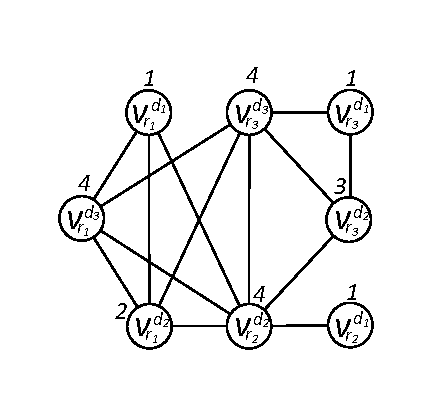
\includegraphics[width=5.5cm]{converted.eps}}
\caption{Example of the Maximum-Weight-Independent-Set problem,
where the number close to a node denotes its corresponding weight.}
\label{Fig:convert}
\end{figure}



For the Maximum-Weight-Independent-Set problem, Sakai et al. propose
an algorithm, called GWMIN2, with an approximation ratio of at least
$\frac{1}{\theta}$ \cite{Sakai2003313}, where $\theta$ denotes the
maximum degree in the given graph $G(V,E,\omega)$. In the GWMIN2, a
cost function is proposed to evaluate the costs of the nodes. The
cost of each node $v \in V$, termed $\phi(v)$, is defined as
follows:

\begin{equation}\label{equa:weigh}
\phi(v) = \frac{\omega (v)}{\sum\nolimits_{u\in N_{G}^{+}(v)}{\omega
(u)}},
\end{equation}
where $N_{G}^{+}\left( v \right)$ denotes the set of $v$ and $v$'s
neighboring nodes in $G$. In the beginning of the GWMIN2, a set $I$
is initialized to be an empty set, and the cost of each node in $G$
must be evaluated with Eq. \ref{equa:weigh}. Then the GWMIN2 is to
iteratively select a node $v$ with maximum $\phi(v)$ in $G$ and add
$v$ to $I$, until no node can be selected. In each iteration, when a
node $v$ with maximum $\phi(v)$ in $G$ is selected, $G$ is updated
as a sub-graph of $G$ induced by $V - N_{G}^{+}\left( v \right)$. In
addition, nodes in $V$ re-evaluate their costs with Eq.
\ref{equa:weigh}.

Take Fig. \ref{Fig:convert}, for example. Initially, $I =
\emptyset$. In the first iteration, because
$N_{G}^{+}(v_{{{r}_{1}}}^{{{d}_{3}}})$ $=$ $\left\{
v_{{{r}_{1}}}^{{{d}_{3}}},v_{{{r}_{1}}}^{{{d}_{1}}},v_{{{r}_{1}}}^{{{d}_{2}}},
v_{{{r}_{2}}}^{{{d}_{2}}},v_{{{r}_{3}}}^{{{d}_{3}}} \right\}$,
applying Eq.\ref{equa:weigh} we have that
$\phi(v_{{r}_{1}}^{{{d}_{3}}})$  $=$ $\frac{4}{4+1+2+4+4}$ $=$
$\frac{4}{15}$. We also have that $\phi(v_{{r}_{1}}^{{{d}_{1}}})$
$=$ $\frac{1}{11}$, $\phi(v_{{r}_{1}}^{{{d}_{2}}})$  $=$
$\frac{2}{15}$, $\phi(v_{{r}_{2}}^{{{d}_{2}}})$  $=$ $\frac{4}{19}$,
$\phi(v_{{r}_{3}}^{{{d}_{3}}})$  $=$ $\frac{4}{18}$,
$\phi(v_{{r}_{2}}^{{{d}_{1}}})$  $=$ $\frac{1}{5}$,
$\phi(v_{{r}_{3}}^{{{d}_{2}}})$  $=$ $\frac{3}{12}$, and
$\phi(v_{{r}_{3}}^{{{d}_{1}}})$  $=$ $\frac{1}{8}$. Therefore,
$\phi(v_{{r}_{1}}^{{{d}_{3}}})$ is the maximum among nodes in the
graph, and node $v_{{r}_{1}}^{{{d}_{3}}}$ is selected and added to
$I$. In addition, the nodes $v_{{r}_{1}}^{{{d}_{3}}}$,
$v_{{{r}_{1}}}^{{{d}_{1}}}$, $v_{{{r}_{1}}}^{{{d}_{2}}}$,
$v_{{{r}_{2}}}^{{{d}_{2}}}$, and $v_{{{r}_{3}}}^{{{d}_{3}}}$ are
removed from the graph. Using the same process, we can add
$v_{{{r}_{3}}}^{{{d}_{2}}}$ and $v_{{{r}_{2}}}^{{{d}_{1}}}$ to $I$
in the second and third iterations, respectively. Finally, we have
that $I=\left\{
v_{{{r}_{1}}}^{{{d}_{3}}},v_{{{r}_{3}}}^{{{d}_{2}}},v_{{{r}_{2}}}^{{{d}_{1}}}
\right\}$. 